%% ============================================================
%% APPENDICES - Supporting Material
%% ============================================================

\clearpage
\appendix
\renewcommand{\thetable}{\Alph{section}.\arabic{table}}
\renewcommand{\thefigure}{\Alph{section}.\arabic{figure}}
\setcounter{table}{0}
\setcounter{figure}{0}
\tightsection{Appendices (Supporting Material)}

\section{Supporting Evidence and Risk Matrix}
\label{app:evidence-risk}
\setcounter{table}{0}
\setcounter{figure}{0}

\begin{table}[H]
\centering
\caption{Asset-focused risk matrix for \texttt{backup01}.}
\label{tab:app-risk-matrix}
\scriptsize
\begin{tabularx}{0.9\linewidth}{L{0.55cm}L{2.9cm}L{1.35cm}L{1.1cm}Y}
\toprule
ID & Risk & Likelihood & Impact & Evidence and uncertainty \\
\midrule
R1 & Unauthorised privileged SSH access via suspected \texttt{backup} credential compromise & High & High & 951 failed passwords from \texttt{203.0.113.89}, followed by accepted \texttt{backup} login. Cannot prove whether the login was authorised without external context. \\
R2 & Escalation to root through \texttt{backup} sudo rights & High & Critical & \texttt{backup} runs sudo as root immediately after login. No destructive root command is visible in auth.log. \\
R3 & Loss of backup-data integrity or availability & Medium & Critical & A root path exists on a backup host. Auth.log does not show backup-file access, exfiltration, or tampering. \\
\bottomrule
\end{tabularx}
\end{table}

\begin{table}[H]
\centering
\caption{Top source IPs by failed authentication attempts.}
\label{tab:app-source-ips}
\footnotesize
\begin{tabularx}{0.82\linewidth}{L{3.1cm}rY}
\toprule
Source IP & Failed & Note \\
\midrule
\texttt{203.0.113.88} & 1,250 & High volume; no accepted login \\
\texttt{198.51.100.88} & 1,100 & High volume \\
\texttt{203.0.113.89} & 951 & High volume + one successful \texttt{backup} login \\
\texttt{198.51.100.89} & 700 & High volume \\
\bottomrule
\end{tabularx}
\end{table}

\begin{table}[H]
\centering
\caption{Most-targeted usernames by failed attempts.}
\label{tab:app-targeted-users}
\footnotesize
\begin{tabularx}{0.82\linewidth}{L{3.1cm}rY}
\toprule
Username & Failed & Relevance \\
\midrule
\texttt{backup} & 1,552 & Sensitive; successful login from \texttt{203.0.113.89} \\
\texttt{root} & 1,048 & Direct privileged targeting \\
\texttt{admin} & 589 & Common admin target \\
\texttt{deploy} & 366 & Operational account \\
\texttt{postgres} & 336 & Service/DB account \\
\texttt{oracle} & 331 & Service/DB account \\
\bottomrule
\end{tabularx}
\end{table}

\begin{figure}[H]
\centering
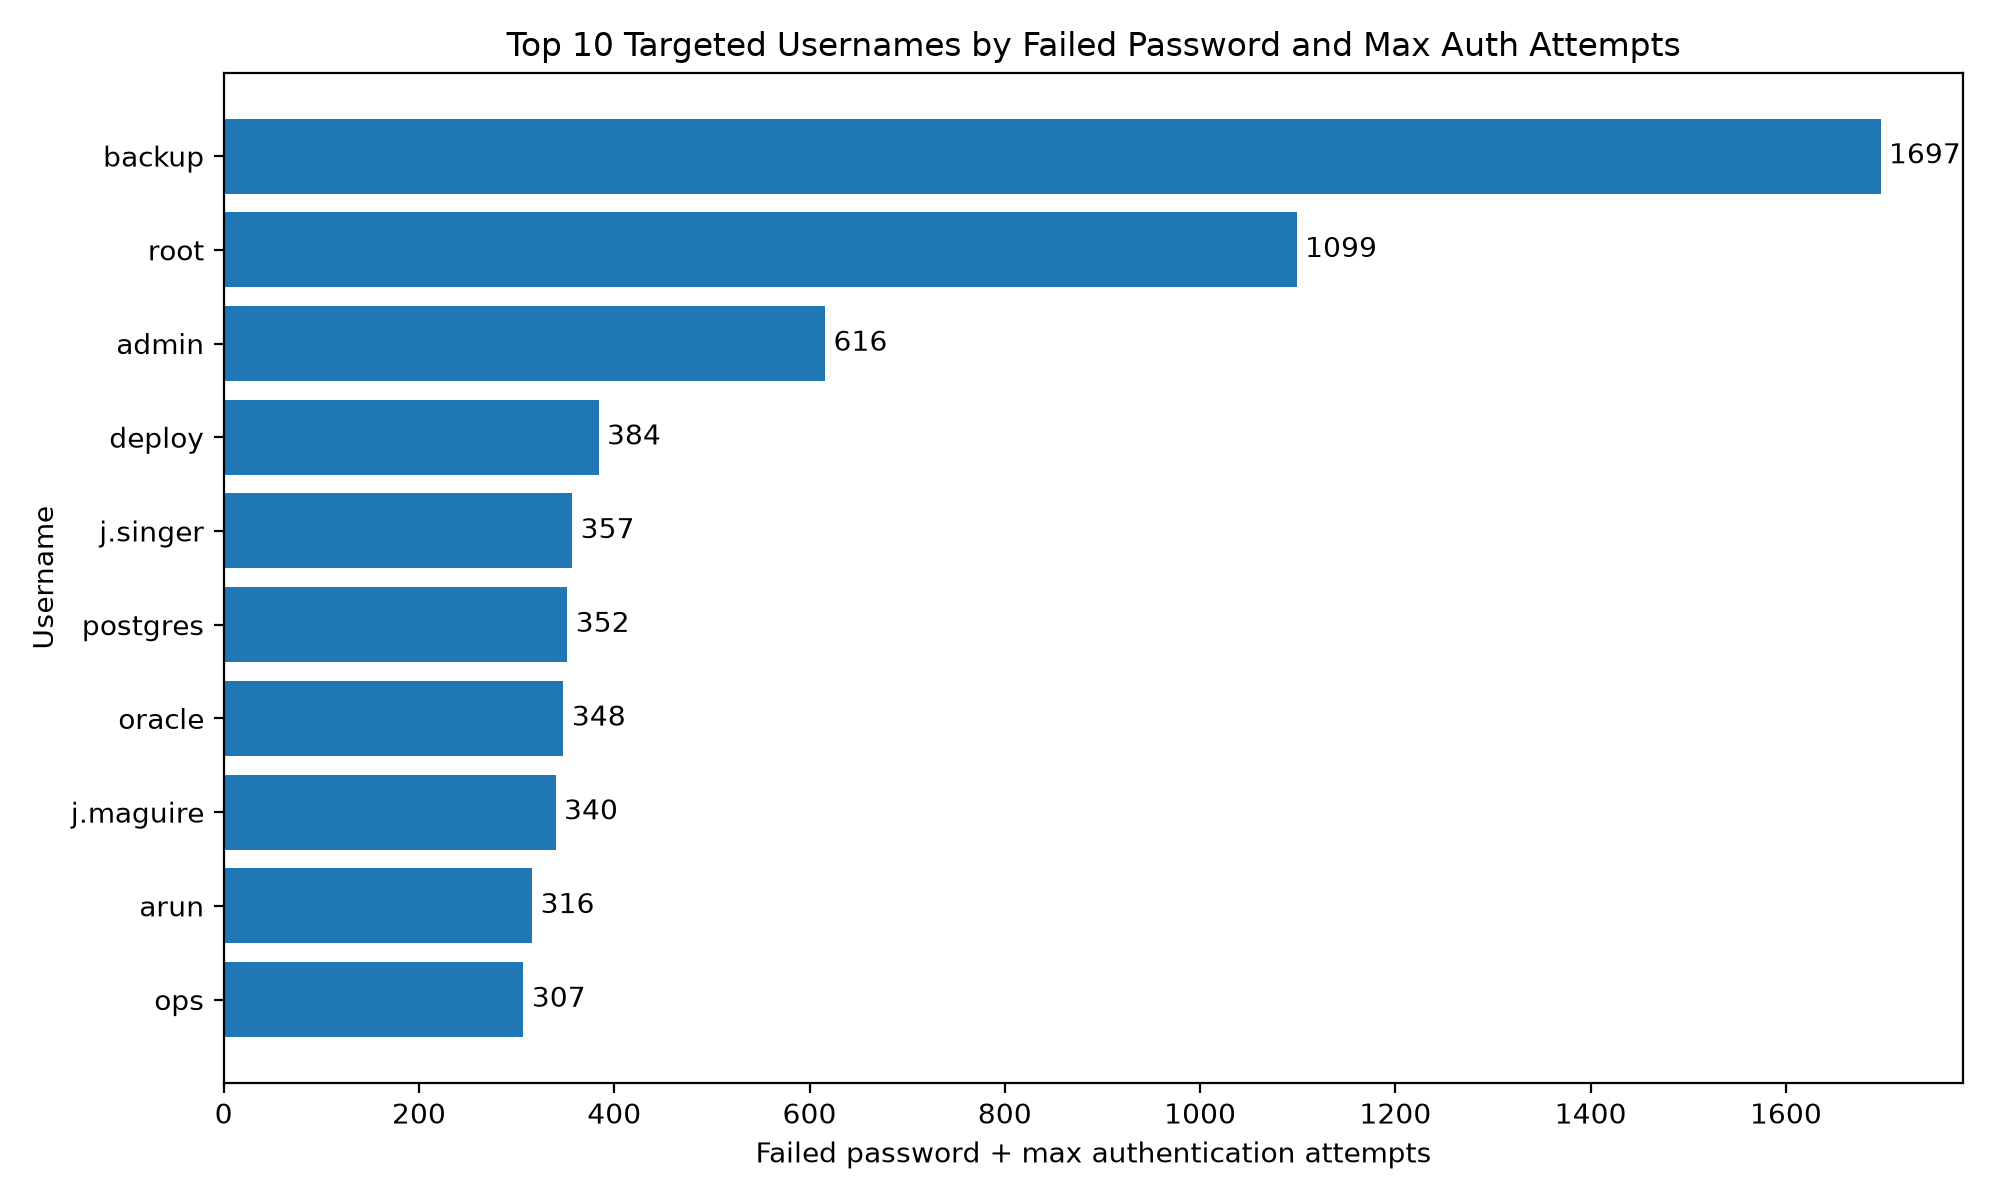
\includegraphics[width=0.62\linewidth]{output/top_targeted_users.png}
\caption{Top targeted usernames by failed-password plus maximum-authentication events. \texttt{backup} is the most targeted account, supporting its selection as the priority privileged asset.}
\label{fig:app-targeted-users}
\end{figure}

\begin{table}[H]
\centering
\caption{Failed vs accepted logins by time window.}
\label{tab:app-time-window}
\footnotesize
\begin{tabularx}{0.82\linewidth}{L{3.0cm}rrY}
\toprule
Window & Failed & Accepted & Note \\
\midrule
Night (00:00--05:59) & 3,643 & 149 & Brute-force concentrated here ($\sim$70\% of all failures) \\
Day (06:00--23:59) & 1,533 & 1,710 & Legitimate activity dominates business hours \\
\bottomrule
\end{tabularx}
\end{table}

Peak failed-login hours are 02:00--04:00; a secondary spike occurs at 23:00. Peak accepted-login hours are 08:00--18:00. The successful \texttt{backup} login (Jul 11 03:08:19) falls inside the peak attack window.

These time-window counts are the Appendix A evidence referenced by the main report for the 03:08:19 off-hours finding.

\begin{table}[H]
\centering
\caption{Timestamp-order anomalies retained as limitations.}
\label{tab:app-timestamp-anomalies}
\footnotesize
\begin{tabularx}{0.9\linewidth}{L{1.0cm}L{2.4cm}L{2.4cm}Y}
\toprule
Line & Previous time & Current time & Interpretation \\
\midrule
13 & 2026-07-06 00:49:51 & 2026-07-06 00:04:24 & Session-close entry appears after later events in file order. \\
41 & 2026-07-06 02:19:09 & 2026-07-06 01:21:46 & Earlier session-close line appears later in the extract. \\
70 & 2026-07-06 03:40:05 & 2026-07-06 02:56:33 & File ordering is not strictly chronological. \\
\bottomrule
\end{tabularx}
\end{table}

\section{Raw Log Excerpt (203.0.113.89, Jul 11)}
\label{app:raw-excerpt}
\setcounter{table}{0}
\setcounter{figure}{0}
\footnotesize
\begin{verbatim}
Jul 11 03:07:30 backup01 sshd[1675]: Failed password for invalid user oracle from 203.0.113.89
port 56854 ssh2

Jul 11 03:07:32 backup01 sshd[1447]: Failed password for root from 203.0.113.89 port 40703
ssh2

Jul 11 03:08:19 backup01 sshd[2164]: Accepted password for backup from 203.0.113.89 port
59595 ssh2

Jul 11 03:08:19 backup01 sshd[7367]: pam_unix(sshd:session): session opened for user backup
by (uid=0)

Jul 11 03:08:19 backup01 sudo: backup : TTY=pts/3 ; PWD=/home/backup ; USER=root ;
COMMAND=/usr/bin/journalctl -n 200

Jul 11 03:08:19 backup01 sudo: backup : TTY=pts/3 ; PWD=/home/backup ; USER=root ;
COMMAND=/usr/bin/systemctl status cron
\end{verbatim}
\normalsize

\section{Parsing Assumptions and Coverage}
\label{app:parsing-coverage}
\setcounter{table}{0}
\setcounter{figure}{0}
\begin{itemize}
    \item Format assumed: Mon DD HH:MM:SS host process[pid]: message; no year in timestamps.
    \item Username handling covers both \texttt{Failed password for USER} and \texttt{Failed password for invalid user USER}.
    \item Non-standard lines (e.g. \texttt{Connection closed by authenticating user ...}, \texttt{reverse mapping ... POSSIBLE BREAK-IN ATTEMPT}) are classified or counted as unmatched, not silently dropped.
    \item Unmatched-line count: 0.
\end{itemize}

\section{AI-Use Declaration and Workload}
\label{app:ai-workload}
\setcounter{table}{0}
\setcounter{figure}{0}
\begin{itemize}
    \item AI-use declaration: Codex GPT-5.5 was used to analyse suspicious points in \texttt{4\_auth.log} so they could be brought to the group's attention for more in-depth analysis. AI was also used to reword and refine the report so that it fits the page limits. Final claims, counts, tables, and figures were checked against \texttt{analysis.py} outputs and the assigned log extract.
    \item Workload record: All members contributed equally.
\end{itemize}
